\section{Le chiffrement asymétrique}
Inventé en 1977 par Diffie et Hellman
\cite{NewDirectionsInCryptography}, le chiffrement symétrique, aussi
connu sous le nom de chiffrement à clé publique permet de résoudre le
problème de communication des clés du chiffrement symétrique, et
permet aussi l'authentification. 

Chaque utilisateur possède alors deux clés : une publique, qu'il
distribue à tout le monde et une privée, qu'il garde secrète. La clé
publique permettra de chiffrer un message, que l'utilisateur pourra
déchiffrer grâce à se clé privée. Ainsi, seul la personne en
possession de la clé de déchiffrement, le destinataire donc, pourra
déchiffrer le message.

Tout chiffrement à clé publique doit répondre aux quatre points
suivants, pour un algorithme de chiffrement $E$, un algorithme de
déchiffrement $D$, une clé quelconque $k$, un message clair $M$ et un
message chiffré $C$ : 
\begin{enumerate}
  \item $E_k$ est l'inverse de $D_k$, donc
    \begin{center}
      $D_k(E_k(M)) = M$
    \end{center}
  \item $E_k$ et $D_k$ sont facile à calculer
  \item $D_k$ est introuvable si l'on connait $E_k$
  \item Si on applique l'opération de déchiffrement suivie de
    l'opération de chiffrement sur un message, on retrouve le message
    d'origine, ainsi
    \begin{center}
      $E_k(D_k(M)) = M$
    \end{center}
\end{enumerate}


\begin{figure}[h]
  \begin{center}
    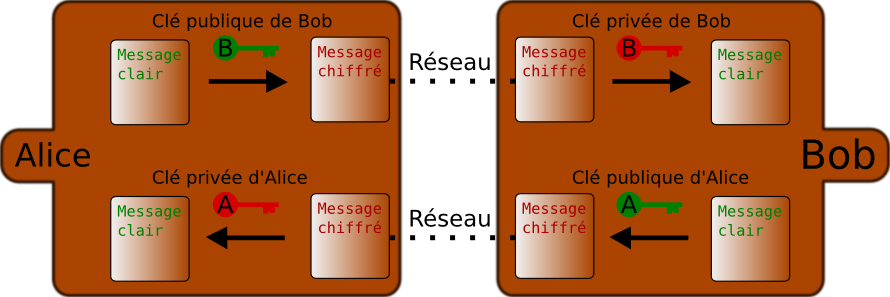
\includegraphics[scale=0.5]{images/ChiffrementAsymetrique.png}
  \end{center}
  \caption{Le fonctionnement du chiffrement asymétrique, pour deux
    échanges de messages entre Alice et Bob.}
  \label{fig:ChiffrementSymetrique}
\end{figure}
